\begin{tikzpicture}
    \def\drawingcode#1#2{
        \begin{scope}[#1]
            \tkzDefPoints{0/0/A#2, 2/0/B#2, 1.8/1/C#2, 0.5/1.3/D#2}
            \tkzDrawPolygon(A#2,B#2,C#2,D#2)
            \tkzDrawSegment[dashed](A#2,C#2)
            \extkzLabelAngel[0.5](B#2,A#2,C#2){$1#2$}
            \extkzLabelAngel[0.4](A#2,C#2,B#2){$2#2$}
            \extkzLabelAngel[0.4](C#2,A#2,D#2){$3#2$}
            \extkzLabelAngel[0.5](D#2,C#2,A#2){$4#2$}
            \tkzLabelPoints[left](D#2)
            \tkzLabelPoints[right](C#2)
            \tkzLabelPoints[below](A#2,B#2)
        \end{scope}
    }

    \drawingcode{scale=1.5}{}
    \drawingcode{xshift=4cm}{'}
\end{tikzpicture}

